% Sezione 3: Requisiti e Selezione Componenti
\section{Requisiti e Componenti}

% Slide 1: Selezione Payload e Requisiti
\begin{frame}
    \frametitle{Selezione Payload}
    \begin{columns}
        \begin{column}{0.48\textwidth}
            \begin{block}{Payload: Compressore a Vite}
                \begin{itemize}
                    \item \textbf{Oggetto}: Compressore Daikin
                    \item \textbf{Peso}: $\sim$730 kg.
                    \item \textbf{Dimensioni}: $1.9 \times 0.9 \times 0.75$ m.
                    \item \textbf{Logistica}: Trasporto da produzione a assemblaggio chiller.
                \end{itemize}
            \end{block}
        \end{column}
        \begin{column}{0.48\textwidth}
            \begin{figure}
                \centering
                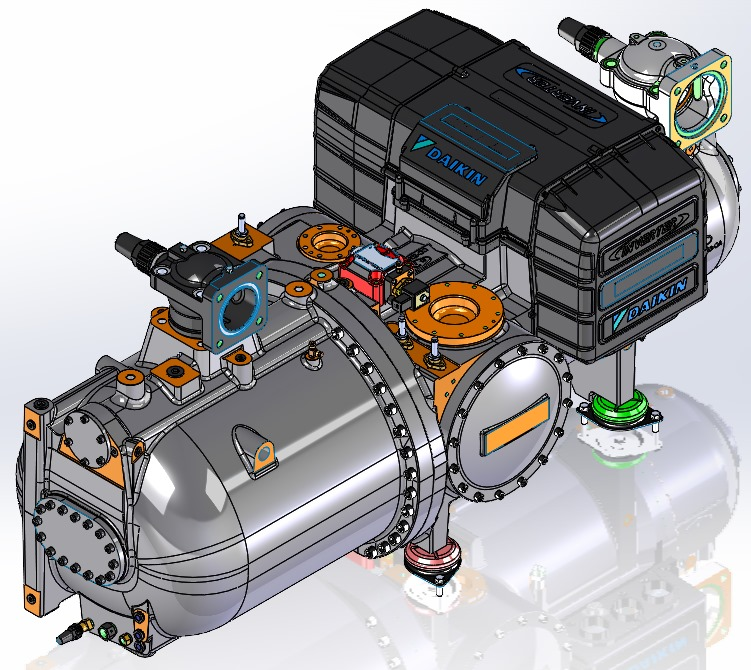
\includegraphics[width=0.6\textwidth]{img/daikin/35-A-CO1005.jpeg}
                \caption{Compressore 35-A-CO1005}
            \end{figure}
        \end{column}
    \end{columns}

    \vspace{0.2cm}
    \begin{alertblock}{Scelta Progettuale}
        Dimensionamento sovrastimato a \textbf{1000 kg} (robot + payload) per scalabilità futura e margine di sicurezza.
    \end{alertblock}
\end{frame}
% Slide 2: Requisiti Veicolo
\begin{frame}
    \frametitle{Requisiti Veicolo}
    \begin{alertblock}{Requisiti Veicolo}
        \begin{itemize}
            \item \textbf{Capacità Carico}: 1000 kg.
            \item \textbf{Velocità Max}: 1 m/s (sicurezza).
            \item \textbf{Autonomia}: 4 ore operative.
            \item \textbf{Ambiente}: Indoor/Outdoor (asfalto, cemento).
            \item \textbf{Manovrabilità}: Omnidirezionale (parcheggio parallelo).
            \item \textbf{Economico}: Costo contenuto per dimostratore tecnologico.
        \end{itemize}
    \end{alertblock}
\end{frame}

% Slide 2: Dimensionamento Potenza
\begin{frame}
    \frametitle{Dimensionamento Potenza}
    Calcolo forza di trazione necessaria ($m=1000$ kg, $v_{max}=1$ m/s):

    \textbf{Parametri:} $\mu_r = 0.03$ (attrito volvente), $\mu_s = 0.5$ (attrito statico), $a = 0.333$ m/s$^2$
    \vspace{0.2cm}
    \begin{columns}
        \column{0.48\textwidth}
        \textbf{In Piano:}
        \begin{equation*}
            \begin{aligned}
                F_r     & = \mu_r \cdot m \cdot g = 294 \text{ N} \\
                F_a     & = m \cdot a = 333 \text{ N}             \\
                F_{tot} & = 627 \text{ N}
            \end{aligned}
        \end{equation*}
        $$P_{piano} \approx 627 \text{ W}$$

        \column{0.48\textwidth}
        \textbf{Pendenza 10\% ($\theta=5.7^\circ$):}
        \begin{equation*}
            \begin{aligned}
                F_{\parallel} & = mg\sin\theta = 974 \text{ N}       \\
                F_r           & = \mu_r mg\cos\theta = 293 \text{ N} \\
                F_a           & = 333 \text{ N}                      \\
                F_{tot}       & = 1600 \text{ N}
            \end{aligned}
        \end{equation*}
        $$P_{salita} \approx \textbf{1.6 kW}$$
    \end{columns}
\end{frame}

% Slide 3: Selezione Batteria
\begin{frame}
    \frametitle{Selezione Batteria}
    \begin{columns}
        \column{0.6\textwidth}
        \textbf{FlashBattery LiFePO4} (Litio-Ferro-Fosfato)
        \begin{itemize}
            \item \textbf{Tensione}: 51.2 V nominali (44-59.2 V).
            \item \textbf{Capacità}: 105 Ah.
            \item \textbf{Energia Totale}: 5.38 kWh.
            \item \textbf{Energia Disponibile} (80\% DOD): \textbf{4.30 kWh}.
            \item \textbf{Corrente}: 105 A continua, 210 A picco.
        \end{itemize}
        \vspace{0.1cm}
        \begin{block}{Verifica Autonomia}
            $$E_{disponibile} = 4.30 \text{ kWh} > 4 \text{ kWh (requisito)}$$
            \textbf{Margine:} 7.5\%

        \end{block}
        \column{0.4\textwidth}
        \centering
        
\includegraphics[width=0.5\textwidth]{batteria/front_view.jpeg}
    \end{columns}
\end{frame}

% Slide 4: Selezione Motori
\begin{frame}
    \frametitle{Selezione Motori: CFR MRT05}
    Configurazione: \textbf{2 Ruote Motrici Sterzanti} (Motorwheels) + 2 Caster (diagonali).

    \begin{columns}
        \column{0.42\textwidth}
        \textbf{Specifiche per ruota:}
        \begin{itemize}
            \item \textbf{Trazione}:
                  \begin{itemize}
                      \item Potenza: 500 W (S2-60min)
                      \item Coppia Nom.: 37 Nm
                      \item Coppia Picco: 180 Nm
                      \item Rapporto riduzione: 1:21
                  \end{itemize}
            \item \textbf{Sterzo}:
                  \begin{itemize}
                      \item Potenza: 300 W
                      \item Coppia: 34 Nm
                      \item Rapporto riduzione: 1:45.56
                  \end{itemize}
            \item \textbf{Encoder}: SIN/COS (FTS1)
        \end{itemize}

        \column{0.54\textwidth}
        {\small
            \begin{block}{Verifica Coppia}
                Raggio ruota: $r = 0.099$ m

                \textbf{Piano:}
                $$\tau_{tot} = F_{tot} \cdot r \approx 62 \text{ Nm}$$
                $$\tau_{ruota} = \tau_{tot}/2 \approx 31 \text{ Nm}$$
                $$\tau_{nom} = 37 \text{ Nm} \Rightarrow \textbf{Margine 18\%}$$

                \textbf{Salita 10\%:}
                $$\tau_{tot} \approx 159 \text{ Nm}$$
                $$\tau_{ruota} \approx 79.5 \text{ Nm}$$
                $$\tau_{picco} = 180 \text{ Nm} \Rightarrow \textbf{OK}$$
            \end{block}
        }
    \end{columns}
\end{frame}
\begin{frame}
    \frametitle{Selezione Motori: CFR MRT05}
    \begin{columns}
        \column{0.4\textwidth}
        \centering
        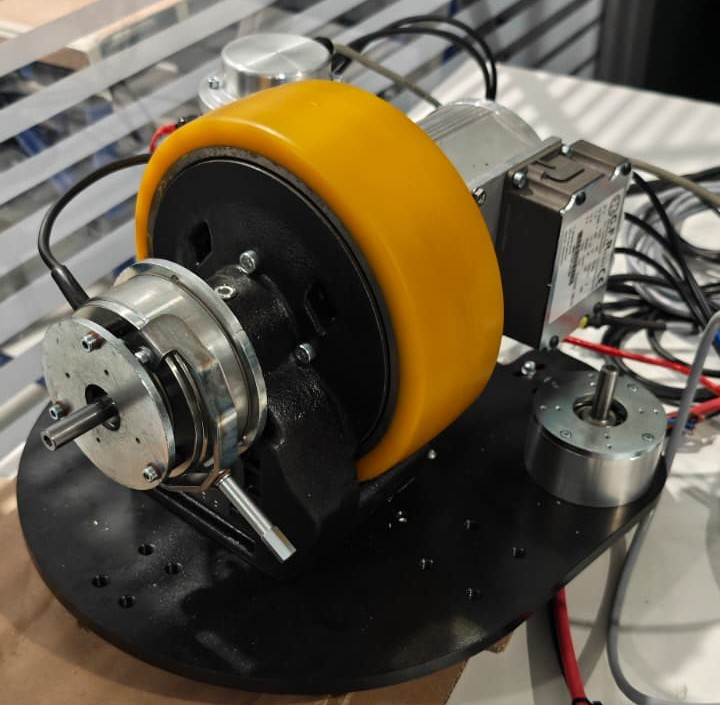
\includegraphics[width=0.8\textwidth]{img/motore/side_view_1.jpeg}
        \column{0.5\textwidth}
        \centering
        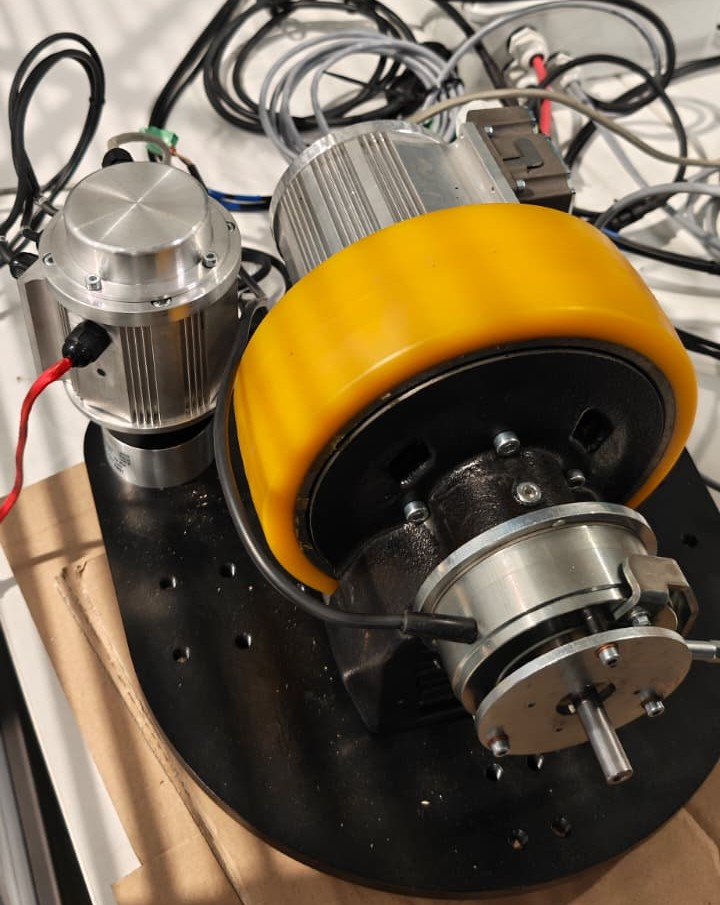
\includegraphics[width=0.6\textwidth]{img/motore/side_view_2.jpeg}
    \end{columns}

\end{frame}
% Slide 5: Architettura Hardware - Parte 1
\begin{frame}
    \frametitle{Architettura Hardware: Computazione e Sensoristica}
    \begin{itemize}
        \item \textbf{Computer di Bordo}: LattePanda Sigma
              \begin{itemize}
                  \item Intel Core i5-1340P (12 core, 16 thread)
                  \item 32GB RAM LPDDR5-6400
                  \item Ubuntu 24.04 + ROS 2 Jazzy
              \end{itemize}
        \item \textbf{LiDAR}: Livox Mid-360
              \begin{itemize}
                  \item FOV: 360° × 59° (-7° a +52°)
                  \item 200k pts/s, portata 70m
                  \item IMU 6-assi integrata (ICM40609)
              \end{itemize}
        \item \textbf{Encoder}: SIN/COS (FTS1) integrati nelle motoruote
        \item \textbf{Sonde Temperatura}: RTD (STS1) per monitoraggio termico motori
    \end{itemize}
\end{frame}

% Slide 6: Architettura Hardware - Parte 2
\begin{frame}
    \frametitle{Architettura Hardware: Alimentazione e Controllo}
    \begin{itemize}
        \item \textbf{Driver Motori}: MicroPhase Mini-Traction Power (4×)
              \begin{itemize}
                  \item Supporto CANopen CiA 402
                  \item 48V, 75A continua, 120A boost (5s)
                  \item Controllo motori PMAC
              \end{itemize}
        \item \textbf{Comunicazione}: Waveshare USB-CAN-A
              \begin{itemize}
                  \item CAN 2.0A/B, velocità fino a 1 Mbps
                  \item Resistenza terminazione 120$\Omega$ commutabile
              \end{itemize}
        \item \textbf{Convertitori DC-DC}: Meanwell
              \begin{itemize}
                  \item SD-25B-12: 48V → 12V, 25W (LiDAR)
                  \item SD-100D-12: 48V → 12V, 102W (SBC)
              \end{itemize}
        \item \textbf{Caricabatterie}: Zivan NG3
              \begin{itemize}
                  \item 48V, 60A configurabile, profilo CC-CV per LiFePO4
                  \item Comunicazione CAN con BMS, tempo ricarica: 2-3h
              \end{itemize}
    \end{itemize}
\end{frame}

% Slide 7: Foto Componenti Hardware
\begin{frame}
    \frametitle{Componenti Hardware}
    \begin{columns}
        \column{0.3\textwidth}
        \centering
        \textbf{LattePanda Sigma}

        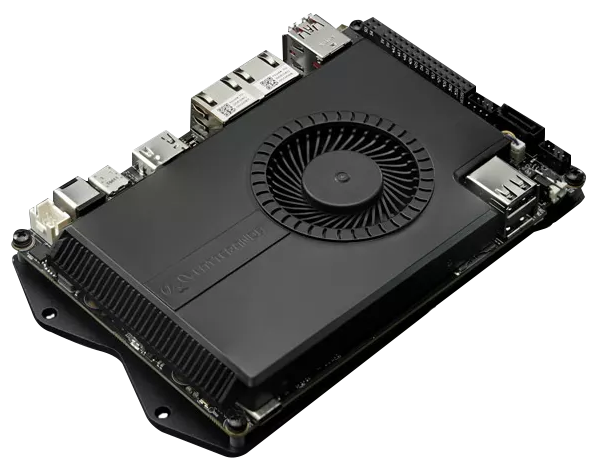
\includegraphics[width=0.7\textwidth]{img/3/lattepanda_sigma2.png}

        \vspace{0.3cm}
        \textbf{Driver Mini-Traction Power}

        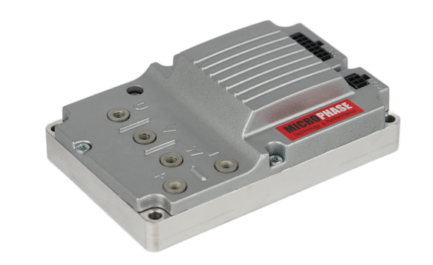
\includegraphics[width=0.7\textwidth]{img/3/mini-traction-power.png}

        \column{0.3\textwidth}
        \centering
        \textbf{Livox Mid-360}

        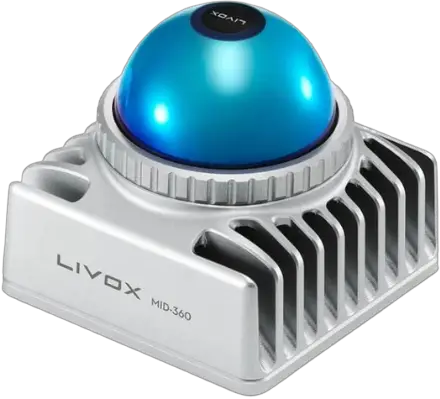
\includegraphics[width=0.6\textwidth]{img/3/livox_mid360.png}

        \vspace{0.3cm}
        \textbf{USB-CAN-A Adapter}

        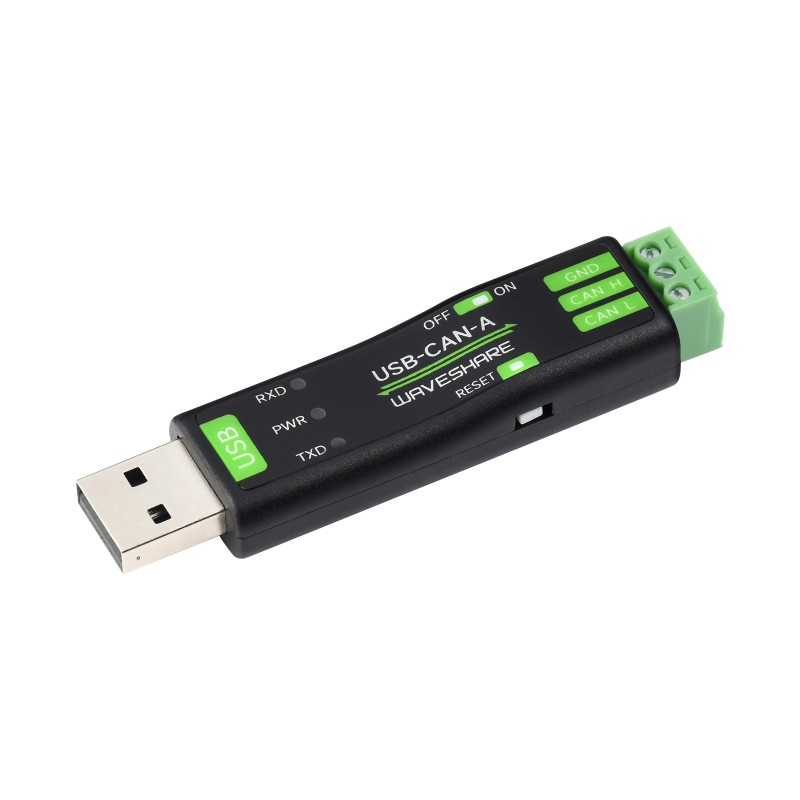
\includegraphics[width=0.6\textwidth]{img/3/usb_can_a.jpg}
    \end{columns}
\end{frame}

% Slide 7: Telaio
\begin{frame}
    \frametitle{Telaio e Struttura Meccanica}
    \begin{columns}
        \column{0.5\textwidth}
        \textbf{Caratteristiche:}
        \begin{itemize}
            \item Massa: $\sim$70 kg
            \item Profili acciaio $30 \times 30 \times 2.6$ mm
            \item Rinforzi $20 \times 20 \times 2$ mm
            \item Dimensioni: $1.8 \times 1.0$ m
            \item Piastre montaggio 5 mm
            \item Trattamento: zincatura
        \end{itemize}

        \vspace{0.3cm}
        \textbf{Progettazione:}
        \begin{itemize}
            \item CAD: SolidWorks
            \item Analisi FEM: FASTRAN
        \end{itemize}

        \column{0.5\textwidth}
        \centering
        
\includegraphics[width=\textwidth]{telaio/disegno_side.png}
    \end{columns}
\end{frame}

% Slide 8: Analisi FEM
\begin{frame}
    \frametitle{Analisi agli Elementi Finiti (FEM)}
    \textbf{Verifica strutturale} con software FASTRAN sotto carico 1000 kg.

    \vspace{0.3cm}
    \begin{columns}
        \column{0.5\textwidth}
        \centering
        \textbf{Mappa delle Deformazioni}

        
\includegraphics[width=0.8\textwidth]{telaio/fem_telaio_dettaglio_3}

        \column{0.5\textwidth}
        \centering
        \textbf{Mappa delle Deformazioni}

        
\includegraphics[width=0.9\textwidth]{telaio/fem_telaio_dettaglio_2}
    \end{columns}

    \vspace{0.3cm}
    \begin{block}{Risultati}
        Deformazioni e tensioni entro limiti di sicurezza. Zone critiche localizzate nei punti di giunzione (artefatti mesh).
    \end{block}
\end{frame}

% Slide 9: Analisi Costi
\begin{frame}
    \frametitle{Analisi dei Costi}
    \begin{table}[htbp]
        \centering
        \small
        \begin{tabular}{|l|r|}
            \hline
            \textbf{Componente}             & \textbf{Costo (€)} \\
            \hline
            Motoruote CFR MRT05 (2×)        & 5.480              \\
            Driver Mini-Traction Power (4×) & 1.640              \\
            Batteria FlashBattery           & 3.950              \\
            Caricabatterie Zivan NG3        & 355                \\
            LattePanda Sigma                & 563                \\
            Livox Mid-360                   & 659                \\
            Telaio, lamierati e caster      & 2.356              \\
            Cablaggi e messa in opera       & 1.800              \\
            Accessori (DC-DC, USB-CAN, SSD) & 429                \\
            \hline
            \textbf{Totale}                 & \textbf{17.232}    \\
            \hline
        \end{tabular}
    \end{table}

    \vspace{0.3cm}
    \begin{block}{Considerazioni}
        Costo contenuto rispetto a soluzioni commerciali (ordine di grandezza inferiore). Dimostratore tecnologico economico per validazione concetto.
    \end{block}
\end{frame}
